\section{Predator-Prey Model}
\numberwithin{figure}{section}
\subsection{Introduction}
ALGEMENE ZEVER

The predator-prey model considered is
\begin{align}
\dot{x} &= x(x-0.2)(1-x) - xy \label{predmodelx} \\
\dot{y} &= xy-by-d \label{predmodely}
\end{align}
in which $b$ and $d$ are physical parameters. The predator dynamics are modeled by $y$ and the prey dynamics are modeled by $x$. The terms in the model each have an ecological interpretation:
\begin{itemize}
\item (\ref{predmodelx}) $x(x-0.2)(1-x)$: The growthfactor of the preys, independent of $y$.
\item (\ref{predmodelx}) $-xy$: The loss of preys, dependent on $y$. The more predators there are, the more preys will be lost.
\item (\ref{predmodely}) $xy$: The growthfactor of the predators, dependent on $x$. When there is more food, the predator population will grow faster.
\item (\ref{predmodely}) $-by$: Natural deaths of the predators.
\item (\ref{predmodely}) $-d$: A control parameter
\end{itemize}
In agreement with the ecological interpretation, only positive values of $x$ and $y$ are considered, unless specifically mentioned otherwise.

\subsection{A qualitative study for $d=0$}
In this section the control parameter $d$ is set to zero, and the parameter $b$ is considered in the region $b \in [0.2,1.5]$.
\subsubsection{The model without predators}
For an impression of the dynamics of the preys without predators, the model is considered for $y=0$. A number of simulations are carried out for initial values $x_0 \in [0,1.5]$. The results are shown in figure \ref{fig:ex3preyonly}. From this figure we can already see that there are 3 fixed points for $y=0$. There is a stable equilibrium for $x=1$, as denoted by the upper red curve. It's basin of attraction is $x_0 \in (0.2,+\infty]$. There is another stable equilibrium at population zero, denoted by the lower red curve, with a basin of attraction $x_0 \in [0, 0.2)$. The point $x=0.2$, denoted by the black curve, is an unstable equilibrium.

The interpretation is as follows: If the initial population is below a certain threshold, it will eventually go extinct. The threshold in this case is $0.2$. If the initial population is anywhere above this threshold, it will evolve to a constant population level 1.
\begin{figure}[htp]
\centering

\includegraphics{img/ex3/preyonly.eps}
\caption{}
\label{fig:ex3preyonly}
\end{figure}
\subsubsection{Steady state solutions and their stability}\label{sec:linearstab}
For the full model (\ref{predmodelx})-(\ref{predmodely}) to have steady state solutions, both $\dot{x}$ and $\dot{y}$ must be zero.
In the previous section we already found that there are three fixed points for $\dot{x}$ when $y$ is zero. As it turns out, $\dot{y}$ is zero too and the fixed points for the model without predators can be carried over to the full model. An additional fixed point is found for $(b,(b-0.2)(1-b))$, with a location dependent of $b$. 

In order to investigate the stability of these four fixed points, the Jacobian matrix $J(x,y)$ is considered as a function of $b$. The eigenvalues of $J$ will determine the stability, so this stability may be dependant on $b$. Note that we only consider $b \in [0.2,1.5]$. 
The Jacobian matrix is given by 
\begin{equation}
J(x,y) = \begin{bmatrix} (x-0.2)(1-x)+x(1-x)-x(x-0.2) & -x \\ y & x-b \end{bmatrix}
\end{equation}
\paragraph{Fixed point $(0,0)$}\hfill\newline
The Jacobian matrix at this point is given by 
\begin{equation}
J(x,y)|_{(0,0)}=\begin{bmatrix}
-0.2 & 0 \\
0 & -b
\end{bmatrix}
\end{equation}
It's eigenvalues are $\lambda_1-0.2$ and $\lambda_2-b$, with corresponding eigenvectors $v_1=(1,0)$ and $v_2=(0,1)$. When both eigenvalues are negative, this fixed point is a stable node. When $b$ is larger than $0.2$, $(1,0)$ will be the slower eigenvector. When $b$ is equal to $-0.2$ the fixed point is a stable star. The behavior of the fixed point is summarized in figure \ref{fig:ex300}.
\begin{figure}[H]
\centering
\subfloat[b=0.2]{
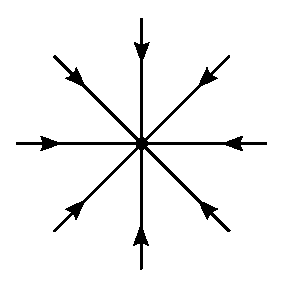
\includegraphics{img/stablestar.eps}}\hspace{18pt}
\subfloat[b>0.2]{
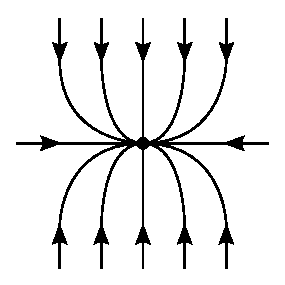
\includegraphics{img/stablenode.eps}}
\caption{}
\label{fig:ex300}
\end{figure}
\paragraph{Fixed point $(0.2,0)$}\hfill\newline
The Jacobian matrix at this point is given by 
\begin{equation}
J(x,y)|_{(0.2,0)}=\begin{bmatrix}
0.16 & -0.2 \\
0 & 0.2-b
\end{bmatrix}
\end{equation}
It's eigenvalues are $\lambda_1=0.16$ and $\lambda_2=0.2-b$, with corresponding eigenvectors $v_1=(1,0)$ and $v_2=(1/(5*(b - 1/25)),1)$. Since one of the eigenvalues is always positive, the fixed point will never be stable. When $b=0.2$, one of the eigenvalues is zero, and the stability cannot be derived from the linearization. A detailed analysis with PPLANE reveals that it is in fact a saddle node, with the stable and unstable manifold determined by the eigenvectors. When $b>0.2$, the fixed point is still a saddle point with unstable manifold $v_1$ and stable manifold $v_2$. The behavior of the fixed point is summarized in figure \ref{fig:ex3020}.
\begin{figure}[H]
\centering
\subfloat[b>=0.2]{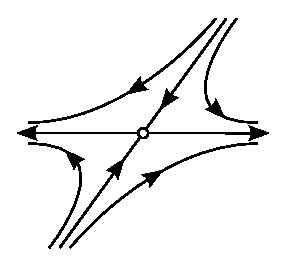
\includegraphics{img/saddle020.eps}}
\caption{}
\label{fig:ex3020}
\end{figure}
\paragraph{Fixed point $(1,0)$}\hfill\newline
The Jacobian matrix at this point is given by 
\begin{equation}
J(x,y)|_{(0.2,0)}=\begin{bmatrix}
-0.8 & -1 \\
0 & 1-b
\end{bmatrix}
\end{equation}
It's eigenvalues are $\lambda_1=-0.8$ and $\lambda_2=1-b$, with corresponding eigenvectors $v_1=(1.8-b,1)$ and $v_2=(0,1)$. When $b \in [0.2,1)$, the eigenvalues have opposite signs and the fixed point is a saddle node with stable manifold $v_1$ and unstable manifold $v_2$. When $b$ equals 1 another borderline case occurs. One of the eigenvalues is zero and the linearization cannot determine the stability.  As detailed analysis with PPLANE shows this fixed point is in fact half-stable, as it undergoes a transcritical bifurcation. When $b \in [1,1.5]$ both eigenvalues are negative and the fixed point is a stable node, with slow eigendirection $v_2$.The behavior of the fixed point is summarized in figure \ref{fig:ex310}.
\begin{figure}[H]
\centering
\subfloat[$b \in [0.2, 1)$]{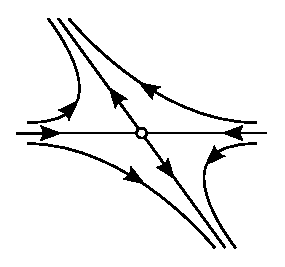
\includegraphics{img/saddle011.eps}}\hspace{18pt}
\subfloat[$b = 1$]{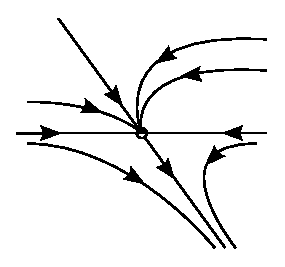
\includegraphics{img/saddle10.eps}}\hspace{18pt}
\subfloat[$b \in (1,1.5)$]{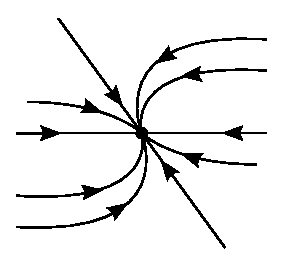
\includegraphics{img/saddle012.eps}}
\caption{}
\label{fig:ex310}
\end{figure}

\paragraph{Fixed point $(b,(b-0.2)(1-b))$}\hfill\newline
The Jacobian matrix at this point is given by 
\begin{equation}
J(x,y)|_{(b,(b-0.2)(1-b))}=\begin{bmatrix}
-2b^2+1.2b & -b \\
(1-b)(b-0.2) & 0
\end{bmatrix}
\end{equation}
Its eigenvalues are less straightforward to compute. They are given by the roots of the quadratic equation 
\begin{equation}
\lambda^2-b(1.2-2b)\lambda+b(1-b)(b-02.)
\end{equation}
The discriminant of this quadratic equation is a function of $b$, and as is mentioned in the assignment has zeros at $b=-.9318$, $b=0$, $b=0.240923$ and $b=0.890889$. The discriminant will change it's sign on every zero, and this will determine wether the eigenvalues have a nonzero imaginary part. A plot of the real and imaginary parts of $\lambda_1$ and $\lambda_2$ is shown in figure \ref{fig:ex3eigvalues}. A plot of the trace and the determinant is shown in figure \ref{fig:ex3tracedeterminant}. As can be seen in figure \ref{fig:ex3eigvalues}, the imaginary parts indeed appear and disappear at the zeros of the discriminant. Furthermore, it is seen that the real parts of the eigenvalues pass through zero several times, so there will be changes in stability.
\begin{figure}[htp]
\centering

\includegraphics{img/ex3/eigvalues.eps}
\caption{}
\label{fig:ex3eigvalues}
\end{figure}
\begin{figure}[htp]
\centering

\includegraphics{img/ex3/tracedeterminant.eps}
\caption{}
\label{fig:ex3tracedeterminant}
\end{figure}
\newline An overview of the changes in topology are given for meaningful values of $b$, again in the interval $b\in[0.2 1.5]$
\begin{description}
\item[$b = 0.2$]\hfill\newline At this point, $Re(\lambda_2)$ changes from negative to positive, so the fixed point has two positive eigenvalues and becomes an unstable node.
\item[$b \in (0.2,0.240923)$]\hfill\newline In this region the fixed point is an unstable node.
\item[$b = 0.240923$]\hfill\newline At this point the eigenvalues of $J$ become imaginary, and the unstable node will bend into an unstable spiral. This is not a bifurcation since the topology is not structurally different. This point is called a degenerate source.
\item[$b \in (0.240923,0.6)$]\hfill\newline In this region the fixed point is an unstable spiral.
\item[$b= 0.6$]\hfill\newline At this point $Re(\lambda_{1,2})$ will turn negative. This is a sign of a Hopf bifurcation (possibly degenerate), and it marks the change from an unstable to a stable spiral.
\item[$b \in (0.6, 0.890889)$]\hfill\newline In this region the fixed point is a stable spiral.
\item[$b = 0.890889$]\hfill\newline At this point $Im(\lambda_{1,2})$ become zero again and the stable spiral becomes a stable node.
\item[$b \in (0.8890889,1)$]\hfill\newline In this region the fixed point is a stable node.
\item[$b=1$]\hfill\newline At this point $Re(\lambda_2)$ will change from negative to positive so $\lambda_1$ and $\lambda_2$ have opposite signs. The stable node will turn into a saddle point. This point engages in a transcritical bifurcation with the fixed point $(1,0)$.
\item[$b\in(1,1.5)$]\hfill\newline In this region the fixed point is a saddle point. 
\end{description}
An overview of the diferent topologies is given in figure \ref{fig:ex3bb}. An overview of the trajectory of this fixed point in function of $b$ is given in figure \ref{fig:ex3trajectory}. This figure shows that for $b=0.2$ and $b=1$ this fixed point will indeed interact with other fixed points, as was seen in the transcritical bifurcation at $b=1$.
\begin{figure}[htp]
\centering
\subfloat[$b \in (0.2,0.240923)$]{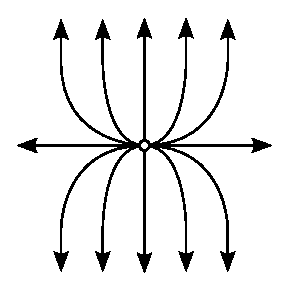
\includegraphics{img/unstablenode.eps}}\hspace{18pt}
\subfloat[$b \in (0.240923,0.6)$]{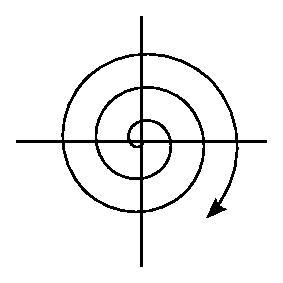
\includegraphics{img/unstablespiral.eps}}\hspace{18pt}
\subfloat[$b \in (0.6, 0.890889)$]{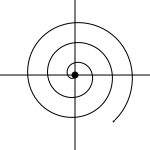
\includegraphics{img/stablespiral.eps}}\\
\subfloat[$b \in (0.8890889,1)$]{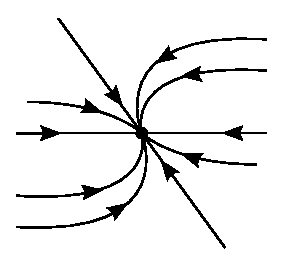
\includegraphics{img/saddle012.eps}}\hspace{18pt}
\subfloat[$b=1$]{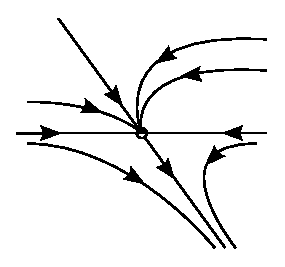
\includegraphics{img/saddle10.eps}}\hspace{18pt}
\subfloat[$b\in(1,1.5)$]{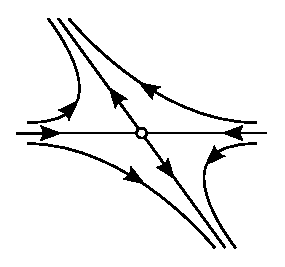
\includegraphics{img/saddle011.eps}}
\caption{}
\label{fig:ex3bb}
\end{figure}
\begin{figure}[htp]
\centering
\includegraphics{img/ex3/btrajectory.eps}
\caption{}
\label{fig:ex3trajectory}
\end{figure}

In order to verify the analysis, some phase diagrams generated with PPLANE are shown in figures \ref{fig:PPLANE1} to \ref{fig:PPLANE5}, for different values of $b$. For increased readability of this report, the diagrams are in appendix.

\subsubsection{Separatrices and regions of attraction}
In order to find the separatrices we must find the boundaries between regions of attraction and regions of repulsion. Two different values for $b$ are considered, namely $b=0.5$ and $b=0.65$. 

When $b=0.5$ the phase diagram can be seen in figure \ref{fig:PPLANE1}. Since the spiral is unstable, every initial point with $y>0$ will converge to the stable node at the origin. When $y<0$, there is a boundary between a stable and an unstable region, determined by the stable manifold of the saddle node at $(0.2,0)$. In order to calculate these boundaries, the stable manifold must be simulated backwards from the saddle node. Two problems arise when doing this:
\begin{itemize}
\item The simulation must go backwards. To this end the signs of the derivatives in the model equations (\ref{predmodelx})-(\ref{predmodely}) are flipped. This way the simulation will go backwards in time.
\item The simulation should start on the stable manifold, as close as possible to the saddle point. The initial points are chosen as a small perturbation from the saddle point along the direction of the stable manifold computed in the linearized analysis.
\end{itemize}
The separatrices and regions of attraction for $b=0.5$, along with the stable manifold of the saddle, are shown in figure \ref{fig:ex3separatrices1}.

When $b=0.65$ the phase diagram is shown in figure \ref{fig:PPLANE3}. The spiral has now become stable, and there will be two regions of attraction, one for the stable node at the origin and one for the spiral. The situation for $y<0$ remains the same. The calculations are executed similar to the case $b=0.5$, and the results are shown in figure \ref{fig:ex3separatrices2}
\begin{figure}[htp]
\centering
\subfloat[$b=0.5$]{
\includegraphics{img/ex3/separatrices1.eps}\label{fig:ex3separatrices1}}
\subfloat[$b=0.65$]{
\includegraphics{img/ex3/separatrices2.eps}\label{fig:ex3separatrices2}}
\caption{}
\label{fig:}
\end{figure}
\subsubsection{An overview of the changes in the phase diagram}
A lot of information regarding the stability of the fixed points was already given in section \ref{sec:linearstab}. This section will summarize these results in a qualitative overview of the changes in the phase diagram for varying $b$. More attention will also be given to the bifurcations occuring.

\subsubsection{An important global bifurcation}
As established in the previous section, a supercritical Hopf bifurcation occurs at $b=0.6$. What is not yet established is where the stable limit cycle needed for this bifurcation comes from. A detailed analysis of the phase diagrams for $b \in [0.52 0.57]$ reveals the bifurcation from which the stable limit cycle originates. A help to understanding this bifurcation is the behavior of the stable manifold of the saddle at $(0.2,0)$. When $b<b_{crit}$, the stable manifold will disappear into the unstable spiral.When $b>b_{crit}$, the stable manifold goes off to $+\infty$.  When $b=b_{crit}$, the stable manifold of the saddle point will be connected to the unstable manifold of the saddle point at $(1,0)$ through a heteroclinic trajectory.The evolution of the stable manifold is shown in figure \ref{fig:ex3unstablemanfold}.
\newline
\newline
When $b>b_{crit}$ the heteroclinic trajectory detaches from the saddle points and constitutes a stable limit cycle. In agreement with Strogatz' definition of a homoclinic bifurcation of cycles this can be called a heteroclinic bifurcation of cycles. The stable limit cycle will shrink with increasing $b$, as shown in figure \ref{fig:ex3homoclinicorbits}, until it collapses onto the fixed point for the Hopf bifurcation.
\newline
\newline
Through iterative simulation of the stable manifold it is found that it forms a heteroclinic trajectory at $b\approx0.538$. The phase diagram is shown in figure \ref{fig:PPLANEhomoclinic}.
\begin{figure}[htp]
\centering
\subfloat[unstable manifold]{
\includegraphics{img/ex3/homoclinicmanfold.eps}\label{fig:ex3unstablemanfold}}\hspace{18pt}
\subfloat[limit cycles]{
\includegraphics{img/ex3/homoclinicorbits.eps}\label{fig:ex3homoclinicorbits}}
\caption{}
\label{fig:}
\end{figure}
The period of the limit cycles is very long just after the heteroclinic bifurcation, and becomes shorter and shorter moving towards the Hopf bifurcation. This is because the heteroclinic bifurcation resembles an infinite period bifurcation in the sense that the initial heteroclinic trajectory has an infinite period. The period length for increasing $b$ is shown in Table \ref{tbl:orbitperiod}.  The decreasing of the period is clearly visible. The table shows the results computed with PPLANE, but the accuracy of these results is not known.
\begin{table}[H]
\begin{center}
\begin{tabular}{|l|c|}
  \hline                        
  $b$ & Period(s) \\
  \hline 
  $b_{crit}$ & $\infty$ \\
  0.55 & 35.5 \\
  0.56 & 29.6 \\
  0.57 & 26.1 \\
  0.58 & 23.7 \\
  0.59 & 21.8 \\
  \hline  
\end{tabular}
\end{center}
\caption{}
\label{tbl:orbitperiod}
\end{table}
\begin{figure}[htp]
\centering

\includegraphics{img/ex3/PPLANEhomoclinic.eps}
\caption{}
\label{fig:PPLANEhomoclinic}
\end{figure}
\subsubsection{Evolution of $x$ and $y$ on the limit cycles}
In this section we compare the behavior of the populations $x$ and $y$ on a limit cycle. We compare a limit cycle for $b=0.545$, close to the heteroclinic cycle, and a limit cycle for $b=0.59$ corresponding to an almost harmonic oscillation. The distance between points on the limit cycle for regular time intervals is shown in figure \ref{fig:ex3speeds}. From these distances the speed at a point on the limit cycle can be calculated. In figure \ref{fig:ex3coloredorbits} both limit cycles are shown with a coloration depending on the speed, red being fast and blue being slow. As could already be seen from figure \ref{fig:ex3speeds}, the speed levels out for $b=0.59$.
\begin{figure}[htp]
\centering

\includegraphics{img/ex3/speeds.eps}
\caption{}
\label{fig:ex3speeds}
\end{figure}
\begin{figure}[htp]
\centering

\includegraphics{img/ex3/coloredorbits.eps}
\caption{}
\label{fig:ex3coloredorbits}
\end{figure}
\subsection{Bifurcation analysis}
In this section, the complete bifurcation diagram will be computed with MATCONT, for $b \in[0.1,0.5]$.
\subsubsection{Case $d=0$}
The bifurcation diagram for $d=0$ is shown in figure \ref{fig:ex3bif} for $x$ vs $b$ and $y$ vs $b$. UITLEG OVER BIFURCATIES

The limit cycles computed with MATCONT are shown in figure \ref{fig:ex3dlimitcycles}. This figure indeed shows the heteroclinic bifurcation, with the radius of the limit cycle decreasing until it vanishes in a Hopf bifurcation. 
\begin{figure}[htp]
\centering
\subfloat[$x$ vs $b$]{
\includegraphics{img/ex3/bifx.eps}}
\subfloat[$y$ vs $b$]{
\includegraphics{img/ex3/bify.eps}}
\caption{}
\label{fig:ex3bif}
\end{figure}
\begin{figure}[htp]
\centering

\includegraphics{img/ex3/3dlimitcycles.eps}
\caption{}
\label{fig:}
\end{figure}


\subsubsection{Case $d\ne0$}
\begin{figure}[htp]
\centering
\subfloat[$x$ vs $b$]{
\includegraphics{img/ex3/bifposx.eps}}
\subfloat[$y$ vs $b$]{
\includegraphics{img/ex3/bifposy.eps}}
\caption{}
\label{fig:ex3bifpos}
\end{figure}
\begin{figure}[htp]
\centering
\subfloat[$x$ vs $b$]{\includegraphics{img/ex3/bifnegx.eps}}
\subfloat[$y$ vs $b$]{\includegraphics{img/ex3/bifnegy.eps}}
\caption{}
\label{fig:ex3bifpos}
\end{figure}













